%! TEX root = ../main.tex
\section[The \textsc{Gerda} experiment]{The \textsc{Gerda} experiment}\label{sec:gerda}
\begin{figure}[b!]
	\centering
	\resizebox{\textwidth}{!}{%
	\begin{tikzpicture}[fill=white]
		\node at (0,0) {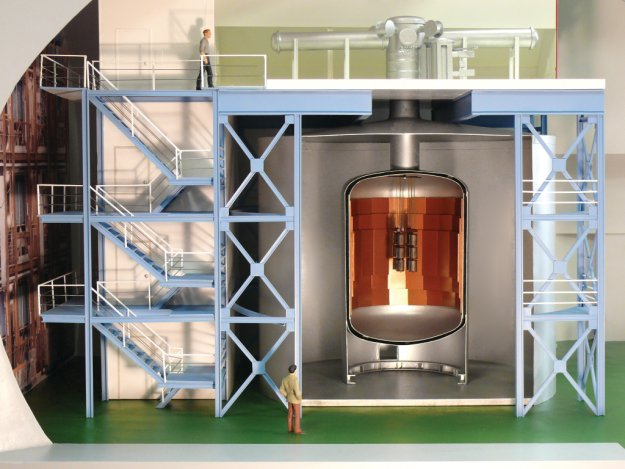
\includegraphics[width=\textwidth]{img/GERDAmodel}};
		\node(a) at (1.9,-1.5) [rectangle,draw,fill] {LAr};
		\node(b) at (4,1.6) [rectangle,draw,fill] {\ce{^76Ge} \textsc{detectors}};
		\draw[thick,red,->] (b.south) .. controls +(0,0) and +(1,0) .. (1.9,-0.4);
		\node(c) at (-1.5,1.6) [rectangle,draw,fill] {\textsc{water tank}};
		\draw[thick,red,->] (c.south) .. controls +(0,0) and +(-1,0) .. (0,-1);
		\node(d) at (0,3) [rectangle,draw,fill] {\textsc{copper shielding}};
		\draw[thick,red,->] (d.south) .. controls +(0,0) and +(-1,0) .. (1,0);
	\end{tikzpicture}%
	\hspace{0.1cm}
	\includegraphics[height=10cm]{img/detectors}%
}
\caption{On the right: artists view (Ge array not to scale) of the {\gerda} experiment. On the left: scheme of the coaxial and BEGe detectors deployed in {\gerda}. On the top the p-type HPGe, on the bottom the BEGe type. The weighting potential is also showed with a color gradient.}
	\label{fig:artistviewanddet}
\end{figure}
% {{{ Introduction
The {\gerda} experiment \cite{gerdadescription} (GERmanium Detector Array) is dedicated to the search of the neutrinoless double-beta decay ($0\nbb$) of \ce{^{76}Ge}. As mentioned in \cref{sec:theory}, the half-lives for $0\nbb$ decay, assuming the process exists, are expected to be substantially longer than the corresponding $2\nbb$ ones, consequently, $0\nbb$ decay experiments must be sensitive to just a few events per year for a source with a mass of tens to hundreds of kilograms. Backgrounds must typically be reduced to the level of one event per year in an energy interval of the order of the energy resolution around $Q_{\beta\beta}$. 

Experiments looking for $0\nbb$ decay of \ce{^{76}Ge} operate germanium diodes normally made from enriched material, i.e.~the number of \ce{^{76}Ge} nuclei, the isotopic fraction $f_{76}$, is enlarged from 7.8\% to 86\% or higher. In these type of experiments, the source is equal to the detector which yields high detection efficiency. Additional advantages of this technique are the superior energy resolution of 0.2\% at $Q_{\beta\beta}=2039$ keV compared to other searches with different isotopes and the high radiopurity of the crystal growing procedure. Disadvantages are the relatively low $Q_{\beta\beta}$ value since backgrounds typically fall with energy and the relative difficulty to scale to larger mass compared to e.g.~experiments using liquids and gases.

{\gerda} has been built in the INFN Laboratori Nazionali del Gran Sasso (LNGS) at a depth of 3500 m w.e.~(water equivalent) and submerses bare high-purity germanium detectors enriched in \ce{^{76}Ge} into liquid argon (LAr). LAr serves simultaneously as a shield against external radioactivity and as a cooling medium. Phase \textsc{i} of the experiment was intended to give a statistically unambiguous statement concerning the observation of the neutrinoless double-beta decay claimed by a subgroup of the \textsc{HdM} collaboration \cite{hdmclaim}. It ended in May 2013 with a total exposure of 21.6 kg$\cdot$yr, and the analysis reported no excess of events above the background at $Q_{\beta\beta}$ \cite{resultsphase1}. More recently the statement was confirmed also by the addition of the first data from Phase \textsc{ii} \cite{nature}, that allowed to reach a 34.4 kg$\cdot$yr exposure and improve the limit on the half-life up to
\begin{equation}T_{1/2}^{0\nu}>5.3\cdot10^{25}\;\text{yr}\qquad\text{(90\% C.L.)}\;.\end{equation}
Phase \textsc{ii} of {\gerda} is expected to further improve the sensitivity up to $10^{26}$ yr.

% }}}
% {{{ DESIGN AND GENERAL LAYOUT
\marginnote{design\\and\\general\\layout} The main feature of the {\gerda} design is to operate bare germanium detectors made out of material enriched in \ce{^{76}Ge} (\ce{^{enr}Ge}) in LAr. It allows for a significant reduction in the cladding material around the diodes and the accompanying radiation sources as compared to traditional germanium experiments. Furthermore, the background produced by interactions of cosmic rays is lower than for the traditional concepts due to the lower atomic number of the shielding material. Other background sources include neutrons and gammas from the decays in the rock of the underground laboratory, radioactivity in support materials, radioactive elements in the cryogenic liquid as well as internal backgrounds in the germanium diodes. Natural Ge (\ce{^{nat}Ge}) contains about 7.8\% \ce{^{76}Ge}, and could in principle be used directly for a $0\nbb$ decay experiment. However enriched detectors allow for a better signal-to-background ratio and also yield reduced costs for a fixed mass of \ce{^{76}Ge} in the experiment.
\begin{figure}
	\centering
	\makebox[0.9\textwidth]{\includegraphics[width=0.9\textwidth]{img/water_tank}}
	\caption{Inside the water tank after the installation of the muon veto system --- August 2009, photo courtesy of Kai Freund ({\gerda} collaboration).}\label{fig:muonveto}
\end{figure}
\begin{figure}
	\centering
	\resizebox{0.9\textwidth}{!}{
		\includegraphics[height=15cm]{img/strings}%
		\hspace{0.1cm}%
		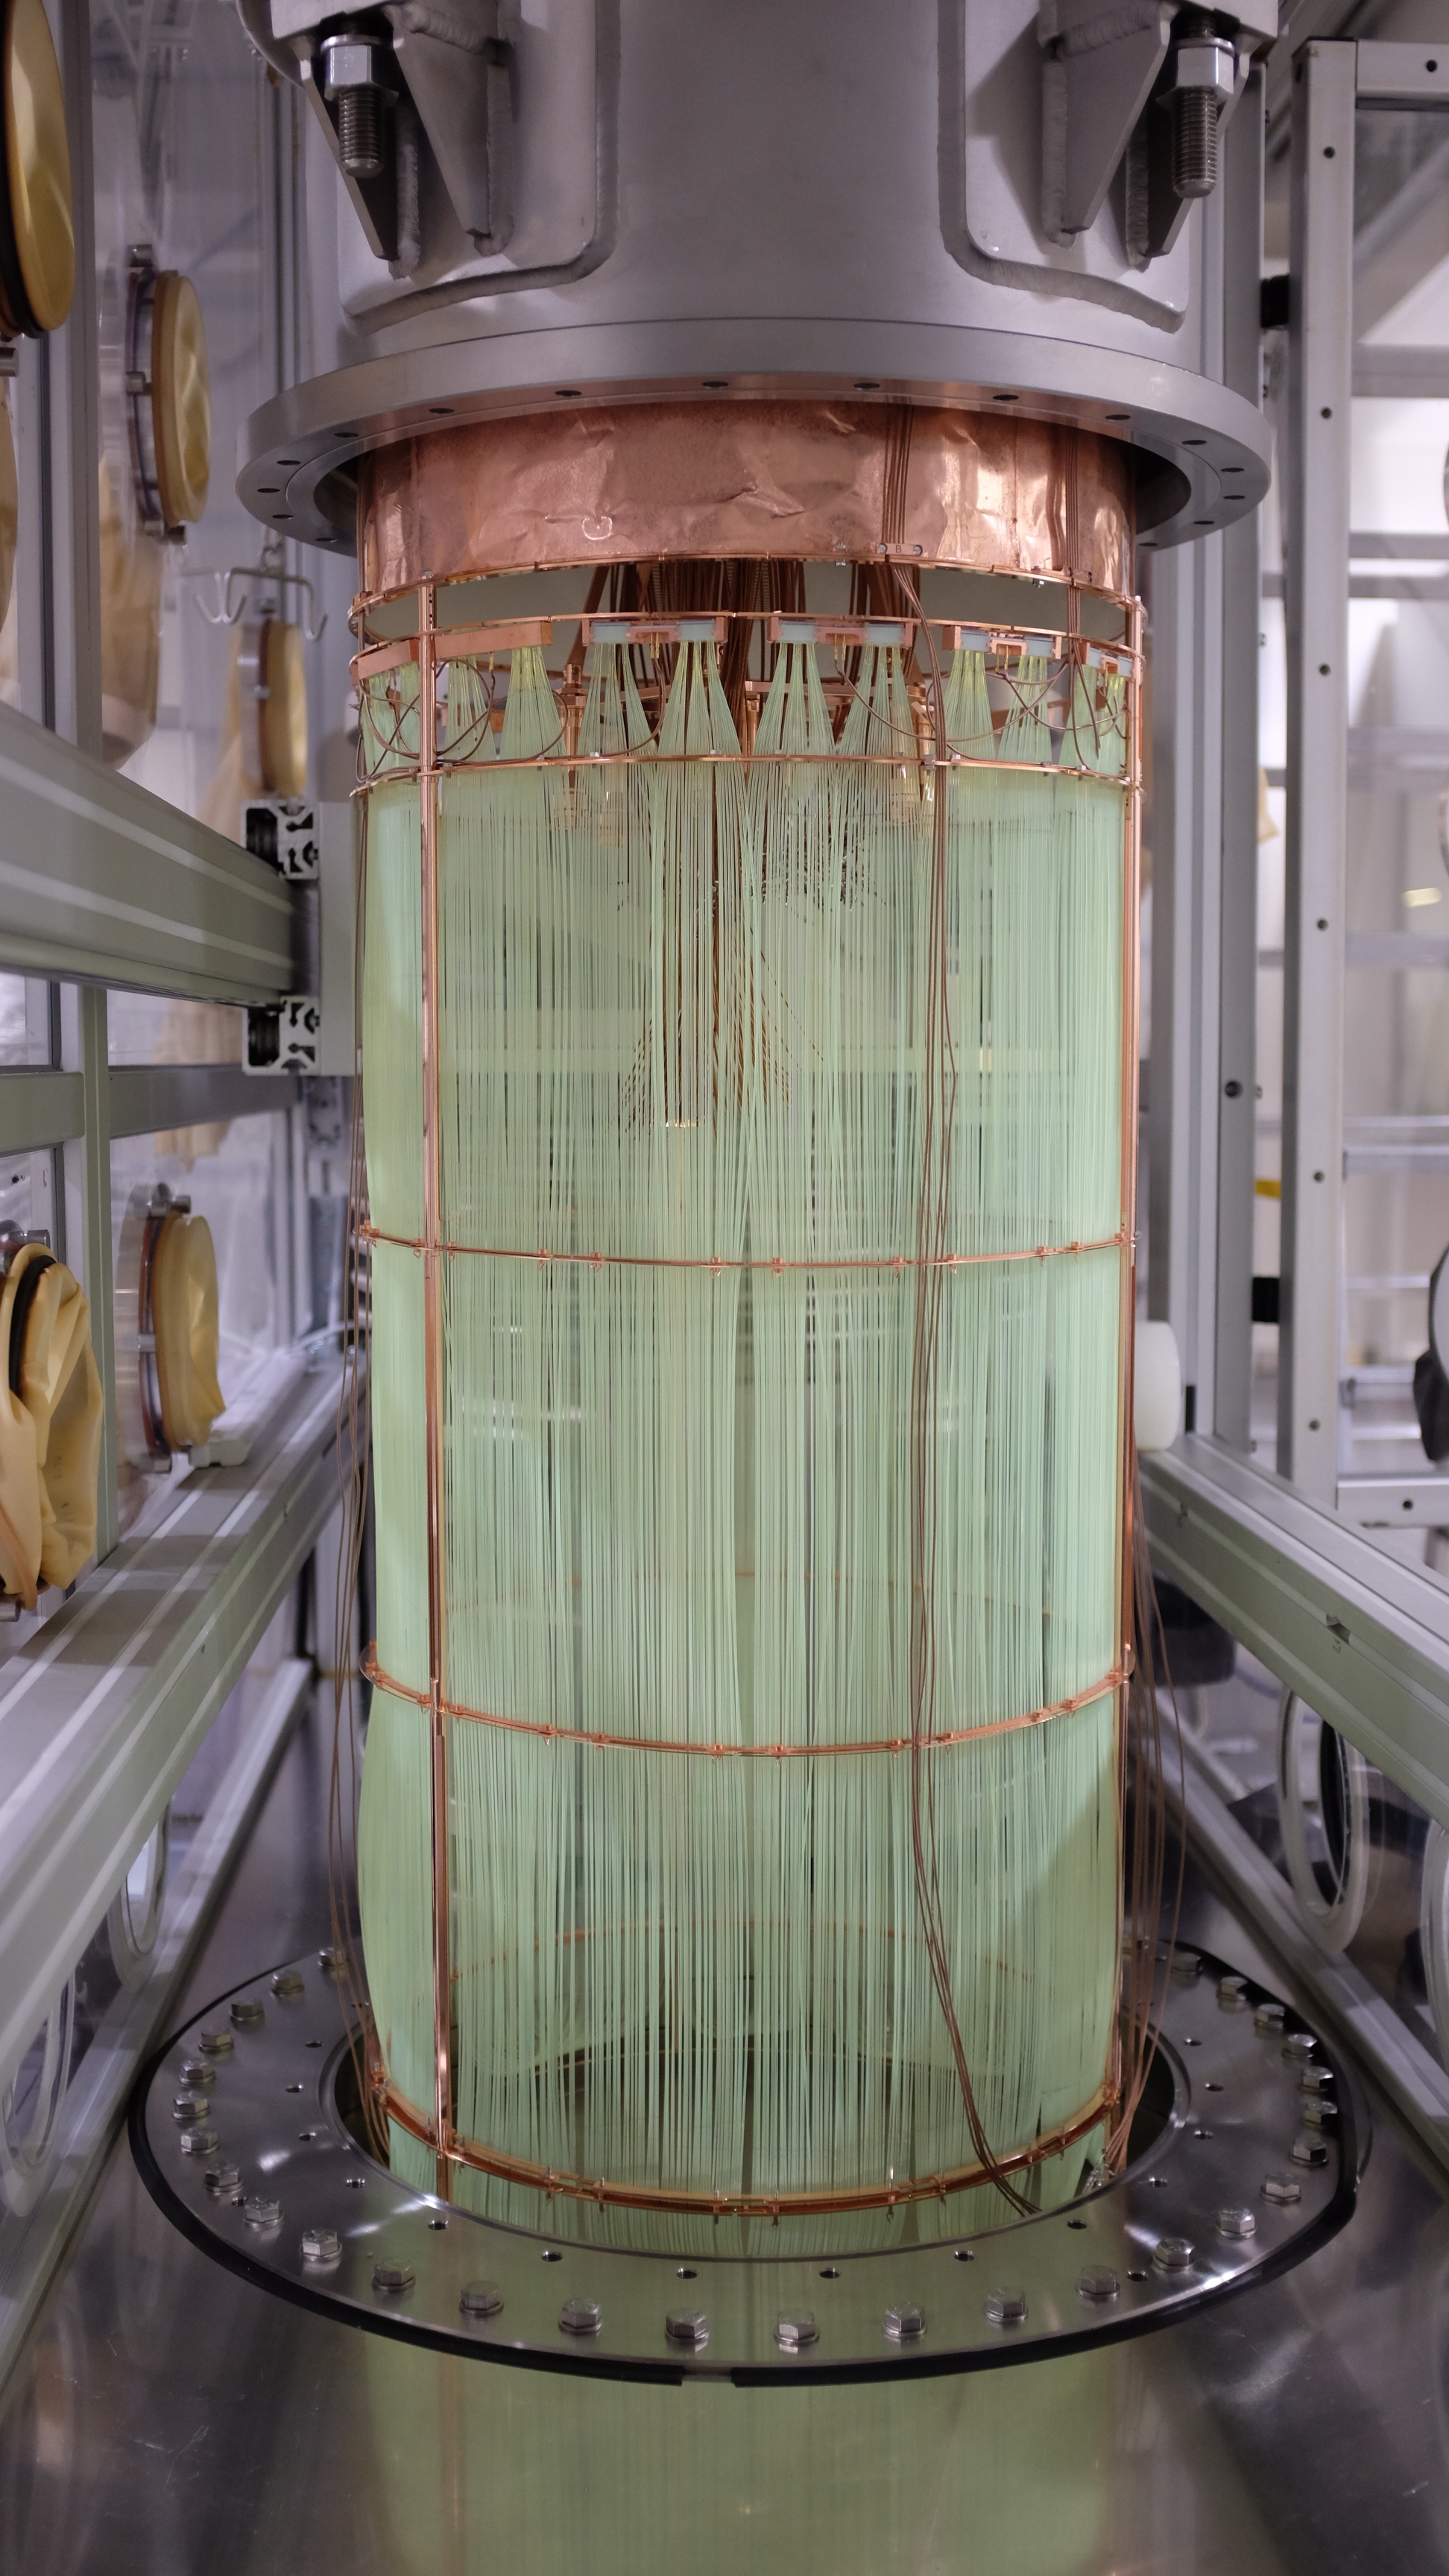
\includegraphics[height=15cm]{img/fibers}%
	}%
	\caption{On the left: some detector strings --- final integration in July 2015, photo courtesy of Bernhard Schwingenheuer. On the right: the fiber-shroud being deployed in LAr --- November 2015, photo courtesy of Mark Heisel.}\label{fig:stringsfibers}
\end{figure}

Fig.~\ref{fig:artistviewanddet} (left) shows a model of the realized design: the core of the experiment is an array of germanium diodes suspended in strings into a cryostat filled with LAr. The LAr serves both as cooling medium and shield. The cryostat is a steel vessel with a copper lining used primarily to reduce the gamma radiation from the steel vessel. The cryostat is placed in a large water tank, that fulfills the functions of shielding the inner volumes from radiation sources within the hall, such as neutrons, as well as providing a sensitive medium for a muon veto system (Fig.~\ref{fig:muonveto}), comprehensive of a set of scintillating panels on the top of the apparatus. The detectors are lowered into the LAr volume using a lock system located in a clean room on top of the water tank. A further muon veto system is placed on top of the clean room in order to shield the neck region of the cryostat. A detailed description of the experimental setup for Phase \textsc{i} is provided in \cite{gerdadescription}.

Phase \textsc{ii} came with some upgrades to improve the background rejection performance. The volume directly surrounding the detector array was instrumented with photo-multipliers to detect the scintillation light emitted if energy is deposited inside LAr. This allows to identify background events resulting from Compton scattered photons with partial energy deposit in the detectors and partial energy deposit inside the LAr. Additionally, a curtain made from light guide fibers with Tetraphenyl butadiene (TPB) deposited on their surface was built to surround the detector array (Fig.~\ref{fig:stringsfibers}, right). Photons reaching the light guides are wavelength shifted and guided to the end of the fibers, where they can be detected by silicon photo-multipliers (SiPMs) optically coupled to the fibers. The new components improve the efficiency in the identification of background events, as proved in \cite{nature}. In Phase \textsc{i} the individual detector strings were surrounded by a copper shroud, minimizing the LAr volume from which \ce{^{42}K} ions, that strongly contribute to the background, can be collected on the detector surfaces. Additionally the shrouds were set to ground potential to minimize drift towards the detectors. In order to take maximum advantage of the light instrumentation of the LAr, in Phase \textsc{ii} the copper shroud has been exchanged by a transparent TPB-coated shroud (called mini-shroud) that allows to minimize the volume from which \ce{^{42}K} ions, that contribute to the background in the \textsc{RoI}, are collected, while allowing to detected scintillation light also from the volume inside the mini-shroud. Last but not least, 30 new BEGe detectors were deployed into the LAr.

% }}}
% {{{ THE GERMANIUM DETECTORS
\marginnote{the\\germanium\\detectors} For Phase \textsc{i} detectors \texttt{ANG1}, \texttt{ANG2}, \texttt{ANG3}, \texttt{ANG4}, \texttt{ANG5} from the \textsc{HdM} \cite{hdm} and \texttt{RG1}, \texttt{RG2}, \texttt{RG3} from the \textsc{Igex} \cite{igex} collaborations were refurbished and redeployed, in addition to three detectors made of \ce{^{nat}Ge} from the GENIUS--TF experiment \cite{genius1, genius2}, \texttt{GTF112}, \texttt{GTF45} and \texttt{GTF32}. A background level of an order of magnitude lower than in those former experiments was achieved. For Phase \textsc{ii} new material was purchased in order to produce new diodes, and another factor of ten in background reduction was accomplished \cite{nature}.

In p-type detectors the dimensionless `weighting potential' $\Phi$ peaks close to the p$^+$ electrode. Ionization creates electrons and holes which drift due to the applied potential and the field created by the space charge of the depleted diode. The time dependent induced current $I(t)$ on the p$^+$ electrode is given by the Ramo-Shockley theorem \cite{schockley-ramo} as:
\begin{equation}I(t)=q\cdot\mathbf{v}(\mathbf{r}(t))\cdot\nabla\Phi(\mathbf{r}(t))\;,\end{equation}
where $q$ stands for the drifting charge and $\mathbf{v}(\mathbf{r}(t))$ for the drift velocity at position $\mathbf{r}(t)$.

Phase \textsc{i} detectors are based on standard p-type HPGe detector technology from Canberra Semiconductor NV, Olen\footnote{Canberra Semiconductors, NV, Lammerdries 25, B-2250, Olen, Belgium; \url{http://www.canberra.com/}}. Standard closed-end coaxial detectors have a `wrap around' $\text{n}^+$ conductive lithium layer ($\sim1$ mm) that is separated from the boron implanted $\text{p}^+$ contact by a groove; the groove region is usually passivated. The detector geometry for one of the enriched detectors is shown schematically in Fig.~\ref{fig:artistviewanddet} (right). In normal DC coupled readout, the p$^+$ contact ($\sim1$ $\mu$m) is connected to a charge sensitive amplifier and the n$^+$ surface is biased with up to +4600 V.

{\gerda} has chosen a modified thick window Broad Energy Germanium (BEGe) detector manufactured by Canberra as the detector type for Phase \textsc{ii}. A batch of 37.5 kg of \ce{^{enr}Ge} was procured by the Electrochemical Plant (ECP) in Železnogorsk, Russia\footnote{Currently known as Joint Stock Company `Production Association Electrochemical Plant' (JSC `PA Electrochemical Plant'), uranium enrichment enterprise of the State Atomic Energy Corporation `Rosatom'.} in 2005 and delivered in the form of \ce{^{enr}GeO2} to the company PPM Pure Metals GmbH\footnote{PPM Pure Metals GmbH, Am Bahnhof 1, 38685 Langelsheim, Germany; \url{http://www.ppmpuremetals.de/.}} in Langelsheim, Germany, to be reduced and further purified. For further zone refinement and crystal growth the 35.5 kg of purified enriched germanium was sent to Canberra Industries Inc.\footnote{Canberra Industries Inc., 107 Union Valley Rd, Oak Ridge, TN, USA; \url{http://www.canberra.com/}}, Oak Ridge (TN), USA. The conversion of the 30 germanium crystal slices into operational BEGe detectors was performed at Canberra Semiconductors NV, Olen, Belgium. Out of 53.4 kg of \ce{GeO2}, containing 37.5 kg of elemental enriched germanium, 30 detectors with a total mass of 20.0 kg were fabricated. One crystal slice (\texttt{GD02D}) turned out to have a non satisfactory impurity distribution. This detector does not reach full depletion and the corresponding voltage plateau; therefore it has a deteriorated charge collection efficiency in some parts of the crystal. Nonetheless, this detector has been deployed in {\gerda} Phase \textsc{ii}; its full or partial inclusion into the analysis can be decided later. Cosmogenically produced isotopes \ce{^{68}Ge} and \ce{^{60}Co} can lead to an internal contamination that represents a background in the region of interest. The detectors are always stored at an underground facility to avoid exposure to cosmic rays\footnote{High Activity Disposal Experimental Site (HADES) of the Belgian Nuclear Research Center SCK$\cdot$CEN, Boeretang 200, BE-2400 Mol, Belgium.}. All the new BEGe detectors were deployed in LAr together with the Phase \textsc{i} detectors during the final integration in July 2015, and \texttt{RG3} was removed from apparatus since it was operated below its full depletion voltage.

Compared to the semi-coaxial detectors used in {\gerda} Phase \textsc{i}, the BEGe detector design shows smaller dimensions and thus smaller mass. Due to a different layout of the electrodes (see Fig.~\ref{fig:artistviewanddet}) the electric field profile in BEGe detectors differs strongly from the one in semi-coaxial detectors. They are made of p-type germanium, comprising a `wrap around' n$^+$ electrode known as `lithium dead layer', a p$^+$ electrode acting as electron blocking contact, and an intercontact insulating surface. For the third item a small annular concentric groove between the p$^+$ and n$^+$ electrodes is produced and covered by an insulating silicon monoxide layer which is known as `passivation layer'. This layer helps to keep steady-state currents (so-called `leakage currents') stable over time. Holes drift to the p$^+$ electrode along the region around the central axis, irrespective of the starting point (`funnel' effect); $I(t)$ peaks at the end of the drift where $\nabla\Phi$ is largest. Hence, the maximum $A$ of $I(t)$ is directly proportional to the deposited energy $E$. Electrons drift through volumes with low $\nabla\Phi$ and hardly contribute to $A$. That means that $A/E$ is constant for all single-site events except for ionizations in a small volume close to the p$^+$ electrode \cite{PSD1, PSD2, PSD3}. In contrast, for multi-site events the drift times of holes from several simultaneous energy depositions are in general different and hence $A/E$ of the summed signal is reduced. For ionizations in the n$^+$ transition layer (like from surface $\beta$-events) the diffusion time is comparable to the drift time and hence $A/E$ is also reduced. For p$^+$ surface events electrons drift through the volume with largest $\nabla\Phi$, and hence $A/E$ is larger than for single-site events due to the increased displacement current. The latter is also the case for events close to the groove. Since it is known that signal events from $0\nbb$ decays deposit energy within a small volume (if the electrons lose little energy by bremsstrahlung), and, on the contrary, in background events energy is often deposited at several locations well separated by a few cm in the detector, the $A/E$ parameter can be used to discriminate between the two situations. A detailed description of the production, characterization and operation of the BEGe detectors in {\gerda} is given in \cite{detectors}, while the pulse shape discriminating techniques adopted for Phase \textsc{i} analysis are presented in \cite{PSDgerda}. Some relevant properties of the detectors deployed in {\gerda} are given in Tab.~\ref{tab:gedet1} and \ref{tab:gedet2}.

The mounting scheme of the detectors has competing requirements. It must have a low mass to minimize sources of radiation near to the detectors. However, the construction must be sufficiently sturdy to provide safe suspension. It must support the cables for detector bias and readout. Furthermore, the diodes must remain electrically isolated from all other materials. The chosen support design can be appreciated in Fig.~\ref{fig:stringsfibers} (left). In order to reach the background goals of {\gerda}, the amount of material is minimized. Only selected high radiopurity materials were used: copper, PTFE and silicon.

% }}}
% {{{ BACKGROUND SOURCES
\marginnote{background\\sources} An important source of background is induced by cosmic radiation. Muon induced background events are efficiently vetoed by identification of Čerenkov light emitted by muons when they pass the water tank or the LAr. The number of long lived cosmogenically produced isotopes, especially \ce{^{68}Ge} and \ce{^{60}Co} are minimized by minimization of the time above ground during processing of the detectors and the structural materials. Further background contributions stem from radioactivity included in the detector and structural materials or the surrounding environment, i.e.~the rocks of the laboratory.

Background from \ce{^{42}Ar} present in LAr was found during {\gerda} commissioning to be more significant than anticipated. The $\beta$-decay of its progeny \ce{^{42}K} can contribute to the background in the \textsc{RoI} if the decay happens near detector surfaces. For coaxial detectors this background was significantly reduced by implementation of the mini-shroud around the germanium strings. However, for the BEGe detectors this remains an important background due to their thinner surface n$^+$ dead layer. The $\beta^-$ decay of the \ce{^{39}Ar} is also a strong component of the energy spectrum, however his Q-value is far below the \textsc{RoI}, at $Q_\beta=565$ keV.

Another potential source of background stems from the calibration sources that have a typical initial activity of about 10–20 kBq. When in parking position they are well shielded and contribute insignificantly.

A significant fraction of the background is induced by contaminations of bulk materials and surfaces with nuclei from the \ce{^{238}U} and \ce{^{232}Th} decay chains. The \ce{^{238}U} decay chain can be subdivided into three sub decay chains: \ce{^{238}U} to \ce{^{226}Ra}, \ce{^{226}Ra} to \ce{^{210}Pb} and \ce{^{210}Pb} to \ce{^{206}Pb}, due to isotopes with half lives significantly longer than the live time of the experiment. Only the two latter sub decay chains are relevant in the following. The noble gas \ce{^{222}Rn} ($T_{1/2} = 3.8$ days) plays a special role, as it can further break the \ce{^{226}Ra} to \ce{^{210}Pb} chain due to its volatility. Whenever activities of \ce{^{214}Bi} are quoted it is assumed that the chain is in secular equilibrium between \ce{^{226}Ra} and \ce{^{210}Pb} inside metallic materials, while for non metallic materials the equilibrium can be broken at \ce{^{222}Rn}.
% }}}
\begin{table}
	\centering
	\caption{Some relevant properties, taken from \cite{GSTR-13-009,GSTR-16-002}, of the detectors deployed in {\gerda} for Phase \textsc{ii}. The mass, the enrichment fraction $f_{76}$, the active volume fraction $f_{av}$ and the FWHM at the \ce{^{208}Tl} peak at 2614 keV are reported. A field is left empty when no information is available.}\label{tab:gedet1}
		{\renewcommand{\arraystretch}{1.3}
	\begin{tabular}{lcccc}
		\toprule
		Detector		&	Mass [g]	&	$f_{76}$	&	$f_{av}$	&	FWHM [keV] \\
		\midrule
		\texttt{GTF32}	&	2321	&	0.087(1)	&	0.97(5)		&	3.49	\\
		\texttt{GTF45}	&	2312	&	0.087(1)	&	--			&	2.86	\\
		\texttt{GTF112}	&	2965	&	0.087(1)	&	--			&	4.36	\\
		\texttt{RG1}	&	2110	&	0.855(15)	&	0.904(59)	&	2.92	\\
		\texttt{RG2}	&	2166	&	0.855(15)	&	0.831(53)	&	2.63	\\
		\texttt{ANG1}	&	958 	&	0.859(29)	&	0.830(52)	&	3.64	\\
		\texttt{ANG2}	&	2833	&	0.866(25)	&	0.871(51)	&	5.42	\\
		\texttt{ANG3}	&	2391	&	0.883(26)	&	0.866(57)	&	2.92	\\
		\texttt{ANG4}	&	2372	&	0.863(13)	&	0.901(57)	&	3.51	\\
		\texttt{ANG5}	&	2746	&	0.856(13)	&	0.831(48)	&	2.88	\\
		\texttt{GD00A}	&	496 	&	0.877(13)	&	0.886$\substack{+0.018\\-0.018}$	&	2.93	\\
		\texttt{GD00B}	&	697 	&	0.877(13)	&	0.880$\substack{+0.018\\-0.017}$	&	3.07	\\
		\texttt{GD00C}	&	815 	&	0.877(13)	&	0.892$\substack{+0.018\\-0.016}$	&	3.12	\\
		\texttt{GD00D}	&	813 	&	0.877(13)	&	0.889$\substack{+0.017\\-0.016}$	&	2.83	\\
		\texttt{GD02A}	&	545 	&	0.877(13)	&	0.896$\substack{+0.015\\-0.014}$	&	2.67	\\
		\texttt{GD02B}	&	625 	&	0.877(13)	&	0.885$\substack{+0.017\\-0.016}$	&	2.81	\\
		\texttt{GD02C}	&	788 	&	0.877(13)	&	0.888$\substack{+0.017\\-0.016}$	&	2.82	\\
		\texttt{GD02D}	&	662 	&	0.877(13)	&	0.834$\substack{+0.016\\-0.016}$	&	2.93	\\
		\texttt{GD32A}	&	458 	&	0.877(13)	&	0.882$\substack{+0.022\\-0.021}$	&	2.61	\\
		\texttt{GD32B}	&	716 	&	0.877(13)	&	0.883$\substack{+0.015\\-0.014}$	&	2.83	\\
		\bottomrule
	\end{tabular}
}
\end{table}
\begin{table}
	\centering
		\caption{Some relevant properties, taken from \cite{GSTR-13-009,GSTR-16-002}, of the detectors deployed in {\gerda} for Phase \textsc{ii}. The mass, the enrichment fraction $f_{76}$, the active volume fraction $f_{av}$ and the FWHM at the \ce{^{208}Tl} peak at 2614 keV are reported.}\label{tab:gedet2}
	{\renewcommand{\arraystretch}{1.3}
	\begin{tabular}{lcccc}
		\toprule
		Detector		&	Mass [g]	&	$f_{76}$	&	$f_{av}$	&	FWHM \\
		\midrule
		\texttt{GD32C}	&	743 	&	0.877(13)	&	0.895$\substack{+0.015\\-0.014}$	&	2.83	\\
		\texttt{GD32D}	&	720 	&	0.877(13)	&	0.913$\substack{+0.016\\-0.014}$	&	3.35	\\
		\texttt{GD35A}	&	768 	&	0.877(13)	&	0.902$\substack{+0.017\\-0.017}$	&	2.83	\\
		\texttt{GD35B}	&	810 	&	0.877(13)	&	0.914$\substack{+0.015\\-0.014}$	&	2.91	\\
		\texttt{GD35C}	&	634 	&	0.877(13)	&	0.902$\substack{+0.016\\-0.015}$	&	2.60	\\
		\texttt{GD61A}	&	731 	&	0.877(13)	&	0.892$\substack{+0.017\\-0.016}$	&	2.95	\\
		\texttt{GD61B}	&	751 	&	0.877(13)	&	0.887$\substack{+0.017\\-0.016}$	&	3.54	\\
		\texttt{GD61C}	&	634 	&	0.877(13)	&	0.887$\substack{+0.017\\-0.016}$	&	2.96	\\
		\texttt{GD76B}	&	384 	&	0.877(13)	&	0.848$\substack{+0.020\\-0.018}$	&	2.96	\\
		\texttt{GD76C}	&	824 	&	0.877(13)	&	0.878$\substack{+0.016\\-0.015}$	&	2.84	\\
		\texttt{GD79B}	&	736 	&	0.877(13)	&	0.881$\substack{+0.019\\-0.018}$	&	3.36	\\
		\texttt{GD79C}	&	812 	&	0.877(13)	&	0.878$\substack{+0.015\\-0.014}$	&	3.97	\\
		\texttt{GD89A}	&	524 	&	0.877(13)	&	0.882$\substack{+0.020\\-0.018}$	&	3.42	\\
		\texttt{GD89B}	&	620 	&	0.877(13)	&	0.859$\substack{+0.020\\-0.019}$	&	2.86	\\
		\texttt{GD89C}	&	595 	&	0.877(13)	&	0.874$\substack{+0.022\\-0.019}$	&	2.90	\\
		\texttt{GD89D}	&	526 	&	0.877(13)	&	0.863$\substack{+0.020\\-0.018}$	&	2.83	\\
		\texttt{GD91A}	&	627 	&	0.877(13)	&	0.889$\substack{+0.017\\-0.017}$	&	2.71	\\
		\texttt{GD91B}	&	650 	&	0.877(13)	&	0.889$\substack{+0.017\\-0.016}$	&	2.93	\\
		\texttt{GD91C}	&	627 	&	0.877(13)	&	0.887$\substack{+0.018\\-0.017}$	&	2.53	\\
		\texttt{GD91D}	&	693 	&	0.877(13)	&	0.888$\substack{+0.018\\-0.017}$	&	3.14	\\
		\bottomrule
	\end{tabular}
}
\end{table}
